%課題研究レジュメテンプレート ver. 1.2

\documentclass[uplatex]{jsarticle}
\usepackage[top=20mm,bottom=20mm,left=20mm,right=20mm]{geometry}
\usepackage[T1]{fontenc}
\usepackage{txfonts}
\usepackage{wrapfig}
\usepackage[expert,deluxe]{otf}
\usepackage[dvipdfmx,hiresbb]{graphicx}
\usepackage[dvipdfmx]{hyperref}
\usepackage{pxjahyper}
\usepackage{secdot}

\makeatletter
  \renewcommand{\section}{%
    \if@slide\clearpage\fi
    \@startsection{section}{1}{\z@}%
    {\Cvs \@plus.5\Cdp \@minus.2\Cdp}% 前アキ
    {.5\Cvs \@plus.3\Cdp}% 後アキ
    %{\normalfont\Large\headfont\raggedright}}
    {\normalfont\raggedright}}

  \renewcommand{\subsection}{\@startsection{subsection}{2}{\z@}%
    {\Cvs \@plus.5\Cdp \@minus.2\Cdp}% 前アキ
    {.5\Cvs \@plus.3\Cdp}% 後アキ
    %{\normalfont\large\headfont}}
    {\normalfont}}

  \renewcommand{\subsubsection}{\@startsection{subsubsection}{3}{\z@}%
    {\Cvs \@plus.5\Cdp \@minus.2\Cdp}%
    {\z@}%
    %{\normalfont\normalsize\headfont}}
    {\normalfont}}
\makeatother
%ここから上を編集する必要はない.

\title{\vspace{-14mm}高齢者入居施設における利用者管理システムの導入}
\author{PMコース 矢吹研究室 1442068 鈴木博文}
\date{}%日付を入れる必要はない.
\pagestyle{empty}%ページ番号は振らない.
\begin{document}
\maketitle

\section{研究の背景}

現在の日本では少子高齢化が大きな課題の一つとなっている.我が国の総人口は,2048年には1億人を割り,2060年には8,000万人になるものと見込まれている.この人口減少と反比例して高齢人口は2010年の2,900万人から団塊の世代及び第二次ベビーブーム世代が高齢人口に入ったあとの2042年に3,800万人とピークを迎えるものとされている.そのため,高齢化率は2013年には25.1\%で4人に1人を上回り,50年後の2060年には39.9\%すなわち2.5人に1人が65歳以上になることが見込まれている.このことから我が国は,人口減少と少子高齢化の急速な進展が現実のものとなることが予測されている\cite{site1}.

高齢化率が上昇するとともに,特別養護老人ホームなどの介護が必要な高齢者が入居する施設が不足しているという点も課題の一つとされている.現在の特別養護老人ホームの入居待ちは,全国で50万人を超えるとされており,行き場のない高齢者は制度外の施設に流れるなど,一般的な老人ホームも全国で不足しているというのが現状だ\cite{site2}.

現状あるホーム内においても満足な経営状況で運営されているとは限らない.介護職員不足に悩まされている施設も多くある.厚生労働省は2025年に介護職員が全国で約38万人不足するという推計を発表している.同年は団塊の世代が75歳以上となる年であり,要介護者の数も相当な数になることが予想される.介護職員が必要な人数に対し,実際に働くことのできる人数は何人かという充足率の統計を見ると,2017年度には94\%となり,早くも6\%の介護者が不足するという推計がでている.この数字は2025年には85.1\%まで低下すると推計されているのだ\cite{site3}.

わたしは,介護者不足と高齢者入居施設不足の問題を並行して解決するためには,少ない人数で現状の作業を効率よく行なうことが必要だと考え高齢者入居施設にWebアプリケーションを用いた利用者の管理ツールを導入することを考えた.

多くの施設では入居者に関する日常の記録は手書きで残しており,過去のデータを含めると非常に多くの紙媒体が保管されている.また,日中に記録されたデータは夜間に集計されることではじめて入居者一人ひとりの一日のデータとなるなど非常に多くの作業を要する.これをWebアプリケーションに置き換えることでスマートフォンやタブレット端末,コンピュータなど様々な端末からアクセスができ,同時に双方向から記録することが可能となる.また,集計を自動化するほか,ヒューマンエラーによる入力漏れや誤入力を防止する.

今回はデザイン科学科の学生との共同作業とし,アイコンなどを用いることによってより分かりやすくし,シンプルで操作しやすい画面デザインを提案する.

\section{研究の目的}

現状で高齢者の入居施設に介護ソフトが導入されている例はあるが,使いづらいなどの理由から機能を使いこなすことが出来ず,場合によってはソフトの使用をやめてしまうという事案が発生していることもある.そのため既存の手書きによるデータ収集よりも手間がかかることがある.これらの課題を解決するため,実際の介護施設での調査を基に新たな利用者管理のシステム開発・提案を行い,IT技術の面から福祉を変えるきっかけとなるのを目指す.今回は実際の高齢者入居施設で記録の方法や問題点,実際にシステム化する場合に便利なる点や留意点などを調査し汎用的なものではなく,調査施設独自の専用のシステムを開発することとする.

\section{プロジェクトマネジメントとの関連}

当研究はPMBOKにおいてプロジェクト・スコープ・マネジメントと関連すると考える.プロダクトを作るにあたってステークホルダが必要とする成果物を納品するためにツールと技法にインタビューを用いるためである.インタビューは,ステークホルダと直接会話をすることによって必要な情報を引き出す.今回のプロダクトは調査する施設独自の専用のシステムを開発することからステークホルダが本当に必要であると考える機能や要求を直接聞くことが重要であると考える.

\section{研究の方法}

\begin{wrapfigure}[5]{r}{8cm}
\vspace*{-\intextsep}
%\includegraphics[width=図の幅,clip]{ファイル名}\label{参照用ラベル}
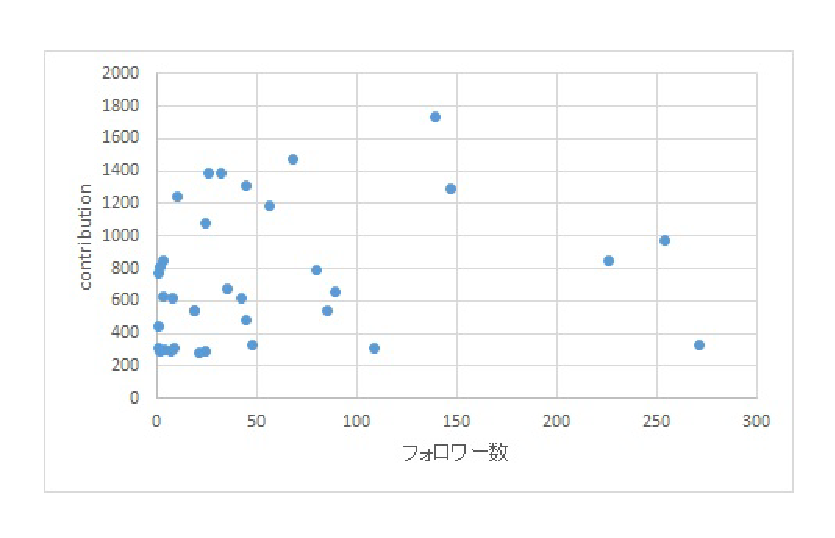
\includegraphics[width=8cm,clip]{figure.pdf}
\caption{アーキテクチャ図}\label{アーキテクチャ}
\end{wrapfigure}

\subsection{システムの構築環境}

当システムはHTML・CSS・JavaScript・PHPの4つの言語を用いる.画面設計はiPad mini(2012)をベースとする.利用者の管理情報はデータベース上に記録され,必要に応じて検索を用いた部分的な抽出や全体の抽出などを行なう.

図\ref{アーキテクチャ}は本システムのアーキテクチャを示す.

\subsection{ハイレベルな要求事項}

\begin{enumerate}
\item 入力値の異常を使用者に的確に知らせ,入力漏れや誤入力を防止する.
\item 機器操作を不慣れとする人にも操作しやすい画面設計とする.
\item 実際の現場で使用するにあたり,使用頻度の高い項目を重点的にシステム化する.
\end{enumerate}

\subsection{プロダクトの評価}

当システムは実際の高齢者入居施設に勤務する介護スタッフ・看護師記録を担当とする方々に実際に使用してもらう.ソフトの基本動作の説明を行い,実際に操作を行ってもらう.その様子を観察するとともに操作後に使用の感想や改善点を再度インタビューし調査対象の施設で使用するにあたって,より独自性の高いシステムを開発する.

\section{現在の進捗状況}

協力をしていただける高齢者入居施設にシステム化すべき項目を聴き,実際にシステムを開発した.16年11月中旬に開発したシステムを協力施設にて担当者に説明を行い一部運用,改善すべき点と評価点をインタビューした.その後改善点を中心にシステムを変更.新規で追加すべき項目を洗い出しシステム開発を継続中である.

\section{今後の計画}

\begin{enumerate}
\item 12月中旬に協力施設を訪問.再度インタビューを行なう.
\item 1月中旬を目処にシステム全体の推移とデータ管理を完成させる.
\item 2月上旬にシステムを完成させる.
\end{enumerate}

\bibliographystyle{junsrt}
\bibliography{biblio}%「biblio.bib」というファイルが必要.

\end{document}
